\documentclass[letter, 10pt]{article}
\usepackage[utf8]{inputenc}
\usepackage[spanish]{babel}
\usepackage{amsfonts}
\usepackage{amsmath}
\usepackage[dvips]{graphicx}
\usepackage{url}
\usepackage[top=3cm,bottom=3cm,left=3.5cm,right=3.5cm,footskip=1.5cm,headheight=1.5cm,headsep=.5cm,textheight=3cm]{geometry}


\begin{document}
\title{Taller de Modelos y Métodos Cuantitativos \\ \begin{Large}Implementación: Algoritmo \emph{Clonal Selection} para el problema \emph{Car Sequencing Problem}\end{Large}}
\author{Cristián D. Maureira Fredes.}
\date{\today}
\maketitle

\section{Introducción}
% Una explicación breve de lo que consiste el informe.

\label{sec:introduccion}

\section{Descripción del problema}
%Descripción breve del problema que se va resolver (revisar entrega anterior):
% Objetivo, restricciones blandas y duras, observaciones especiales.
% Modelo matem\'atico. Instancias a usar. 
\subsection{Descripción}
El \emph{Car Sequencing Problem} es un problema de satisfacción de restricciones (CSP), posee la
característica de ser NP-duro~\footnote{
NP-duro es el conjunto de los problemas de decisión que contiene los problemas H
tales que todo problema L en NP puede ser transformado polinomialmente en H.
Esta clase puede ser descrita como conteniendo los problemas de decisión que son
al menos tan difíciles como un problema de NP.}
, además corresponde a un tipo de variación del problema NP-completo \emph{Job-Shop Scheduling},
pero con un uso de razonamiento automatizado, es decir, con un enfoque dedicado a estudiar y comprender
diferentes características del razonamiento, permitiendo así construir programas que le den la posibilidad
a los computadores para razonar en forma autónoma.

Siguiendo la misma idea, es válido señalar que el \emph{Car Sequencing Problem} es un tipo de problema de planificación
de tareas en una línea de ensamblaje de autos, donde cada uno es perteneciente a un clase de automóvil, debido al conjunto
de opciones y accesorios que posee (airo acondicionado, centralizado eléctrico, etc), y cada una de las opciones o
accesorios se instala en una planta distinta, por lo que el objetivos principal es el poder encontrar el orden en la
secuencia de los vehículos, preocupándonos de no exceder la capacidad de cada planta de ensamblaje y también cumplir con la demanda.

Por lo tanto, si realizamos una definición más formal de nuestro problema, podríamos decir lo siguiente:
Teniendo una lista de vehículos dada, cada uno con sus respectivas opciones requeridas,
necesitamos establecer un orden en la línea de ensamblaje, con el fin de que cada subsecuencia de $q$ vehículos
tengamos a lo más $p$ que requieren de una determinada opción. Es importante tener en consideración que los
valores de $p$ y $q$ están asociados a cada opción de los vehículos.

Con respecto a la información que el problema otorga, podemos decir que contamos con:
\begin{itemize}
    \item Cantidad de vehículos de cada tipo o clase a producir (demanda)
    \item Lista de las opciones con la cual se constituye cada tipo o clase de vehículo, la cual puede utilizar una representación
        booleana para saber si cierto tipo de automóvil posee o no una determinada opción.
    \item Capacidad de las plantas que se preocupan de instalar la determinada opción.
\end{itemize}

Nuestro objetivo principal es:
\begin{itemize}
    \item Encontrar un orden en nuestra secuencia, que sirva para minimizar el costo por cada restricción insatisfecha.
\end{itemize}

Con respecto a las restricciones, tenemos que:
\begin{itemize}
    \item En cada subsecuencia de los $q$ vehículos, a lo más pueden haber $p$ que requieran de la opción determinada.
        Donde $p$ y $q$ son valores asociados a cada opción.
    \item La capacidad de cada planta de ensamblaje no puede ser excedida, es decir, cumplir con la demanda de cada automóvil
        sin abusar de una planta determinada.
    \item Por cada tipo de auto, el numero de autos de ese tipo debe ser secuenciado, es decir, todos los automóviles de cada clase
        deben estar presente en una secuencia determinada.
\end{itemize}

El modelo matemático se omite debido a la total similitud con la representación planteada más adelante.

Las instancias utilizadas son las de entregadas por la CSPlib~\cite{CSP},
para el ``Car Sequencing Problem''.~\footnote{revisado al 12 de octubre, 2010}
\begin{itemize}
	\item 10 instancias para 200 vehículos.
	\item 10 instancias para 300 vehículos.
	\item 10 instancias para 400 vehículos.
\end{itemize}

\label{sec:descripcionProblema}

\section{Algoritmo Propuesto}

\subsection{Representación}
% Descripción detallada de la representación elegida.

A continuación se explica la representación del algoritmo implementado,
que consiste en un \emph{Algoritmo Inmune} utilizando \emph{Selección Clonal}.

\subsection{Representación Matemática}

La presente representación, tiene un carácter simplista, y toma la esencia del modelo
matemático señalado en la sección anterior, buscando en éste caso, dar prioridad a la satisfacción
de la restricciones del problema, de una forma más apropiada.

\begin{itemize}
	\item Parámetros
	\begin{itemize}
		\item $cN$: Número total de autos.
		\item $oN$: Número total de opciones disponibles.
		\item $tN$: Número total de tipos/clases de autos.
	\end{itemize}
	\item Variables
	\begin{itemize}
		\item $nMax_{ij}$: Número máximo de autos con la opción $i$ en una subsecuencia $j$.
		\item $n_{ij}$: Número de autos con la opción $i$ en una subsecuencia $j$.
		\item $sMax_{i}$: Tamaño de la subsecuencia $j$ donde deben haber $nMax_{ij}$ autos.
		\item $q_{k}$: Cantidad de autos del tipo/clase $k$.
		\item $types_{il}$: Booleano que indica si la opción $i$ está presente en el auto $l$.
	\end{itemize}
	\item Función Objetivo
	$$FO\ :\ Min\ \sum\limits_{i=1}^{oN} \sum\limits_{l=1}^{cN} \sum\limits_{j=0}^{sMax_{i}} types_{il}\cdot (n_{ij} - nMax_{ij}), \forall n_{ij} > nM_{ij}$$
	\item Restricciones Duras
	$$\sum\limits_{k=1}^{cN} q_{k} = cN$$
	\item Restricciones Blandas
	$$\sum\limits_{i=1}^{oN} \sum\limits_{l=1}^{cN} \sum\limits_{j=0}^{sMax_{i}} types_{il}\cdot n_{ij} \leq nMax_{ij}$$
\end{itemize}
\subsection{Representación en Estructuras de datos}
La presente representación, posee una alta similitud con la representación matemática, buscando así presentar un código simple
con respecto a la satisfacción de restricciones y función objetivo.

\begin{itemize}
	\item Individuos ($\textbf{struct}\ cell$):
				
		Cada célula de nuestra población, corresponde a una secuencia de autos, más algunos atributos del mismo, por lo tanto,
		para representarlo es necesaria una estructura que posee los siguientes atributos:
		\begin{itemize}
			\item $\textbf{int}\ gene[VARS]$: Arreglo de enteros que corresponden  a la secuencia de autos, en su respectivo orden.
			\item $\textbf{int}\ fitness$: Corresponde a la aptitud de cada individuo, la cual tiene un valor correspondiente a las unidades
				extra por cada opción que sobrepase al máximo de autos permitidos con una cierta opción en una determinada subsecuencia.
			\item $\textbf{double}\ rfitness$: Corresponde a la aptitud relativa de cada individuo, la cual tiene un valor correspondiente
				a una probabilidad relacionada con su \emph{fitness}, la cual será explicada más adelante cuando se hable de la \emph{Selección de
				individuos}.
			\item $\textbf{double}\ cfitness$: Corresponde a la aptitud acumulativa de cada individuo, la cual tiene un valor correspondiente
				a una secuencia de probabilidades relacionadas con su \emph{fitness}, la cual será explicada más adelante cuando se hable de la \emph{Selección
				de individuos}.
		\end{itemize}

	\item Número máximo de autos por subsecuencia ($\textbf{int}\ numMaxCarOptSeq[N]$):
	
		Corresponde a un arreglo de enteros, que representa el número máximo de autos con la opción determinada, en una subsecuencia se nuestro individuo.


	\item Tamaño subsecuencia ($\textbf{int}\ sizeMaxCarOptSeq[N]$):

		Corresponde a un arreglo de enteros, que representa el tamaño de la subsecuencia donde debe haber un número máximo de opciones en un auto (numMaxCarOptSeq).

	\item Demandas y descripción de los tipos de autos ($\textbf{int}\ types[N][M]$):
	
	Corresponde a un arreglo bidimensional, que posee la siguiente información:
	\begin{itemize}
		\item $[N]$ posee sólo el valor del índice de la cantidad de tipos/clases de autos.
		\item $[M]$ posee el valor del índice anterior para cada tipo/clase , demanda del tipo de auto, y para cada opción si la posee o no (1 o 0).
	\end{itemize}
	\item Constantes:

		\begin{itemize}
			\item \emph{VARS(200, 300, 400)}: Número de autos.
			\item \emph{POP (20)}: Tamaño población
			\item \emph{GENS (500)}: Número máximo de generaciones.
			\item \emph{N (128)}: Variable para crear arreglos determinados.
			\item \emph{clonationRate (POP*0.4)}: Tasa para realizar la clonación.
			\item \emph{selRate (POP*0.4)}: Tasa para la cantidad de elementos seleccionados.
			\item \emph{replaceRate (POP*0.6)}: Tasa para la cantidad de elementos reemplazados.
			\item \emph{swap (VARS*0.4)}: Cantidad de swap realizados en el movimiento.
			\item \emph{clonationFactor (0.5)}: Factor para calcular individuos clonados.
		\end{itemize}

\end{itemize}

\label{sec:representacion}

\subsection{Técnica}
% Breve descripción de la técnica que utilizará para resolver el problema, descripción del algoritmo base a utilizar.

\subsection{Origen biológico}

El principio de selección clonal es un modelo que explica la forma en la cual el sistema inmune
responde a una determinada infección y como algunos tipos de linfocitos T y B son seleccionados
para destruir un determinado antígeno que está invadiendo el cuerpo del sujeto.

Fue propuesto por el virólogo australiano, Sir Frank Macfarlane Burnet en el año 1959,
con un trabajo titulado \emph{``The clonal selection theory of acquired immunity''}.

Existen cuatro postulados fundamentales en la hipótesis de la selección clonal, los cuales son detallados más adelante:
\begin{enumerate}
	\item Cada linfocito soporta un solo tipo de receptor con una única especificación.
	\item La ocupación del receptor es requerida para la activación de la célula.
	\item Las células efectoras diferenciadas derivadas desde un linfocito activado soportarán receptores de una especificación idéntica al de la célula padre.
	\item Aquellos linfocitos que soportan receptores para moléculas propias serán eliminados en una etapa temprana.
\end{enumerate}

De acuerdo a la teoría propuesta por Burnet, el repertorio del sistema inmune se somete a un mecanismo de selección durante el tiempo de vida de un individuo.
La teoría establece que al unirse con un antígeno adecuado, se produce la activación de los linfocitos.
Una vez activado, los clones de los linfocitos son producidos con receptores idénticos a los linfocitos originales que encontraron el antígeno.
Así ocurre una expansión clonal de los linfocitos originales.
Esto asegura que solo los linfocitos específicos que se han activado gracias a un antígeno sean producidos en grandes cantidades.
La teoría de la selección clonal también establece que cualquier linfocito que tenga receptores de antígenos de moléculas propias del organismo
debe ser eliminada durante el desarrollo de los linfocitos.
Esto asegura que solo los antígenos de un patógeno pueden causar que un linfocito se clone y se expanda y así generar una respuesta inmune adaptativa a
agentes externos.
Durante la expansión clonal de linfocitos B, el promedio de la afinidad entre los anticuerpos aumenta para el antígeno que desencadena la expansión clonal.
Este fenómeno se llama maduración de la afinidad, y es responsable de el hecho de que en una posterior exposición al antígeno, la respuesta inmune es más eficaz debido a los anticuerpos con una mayor afinidad por el antígeno.
La maduración de la afinidad es causada por una hiper-mutación somática y un mecanismo de selección que ocurre durante la expansión clonal de linfocitos B.
La hiper-mutación somática altera la especificación de los anticuerpos, introduciendo cambios aleatorios a los genes que lo forman.
\begin{figure}[h!]
\begin{center}
%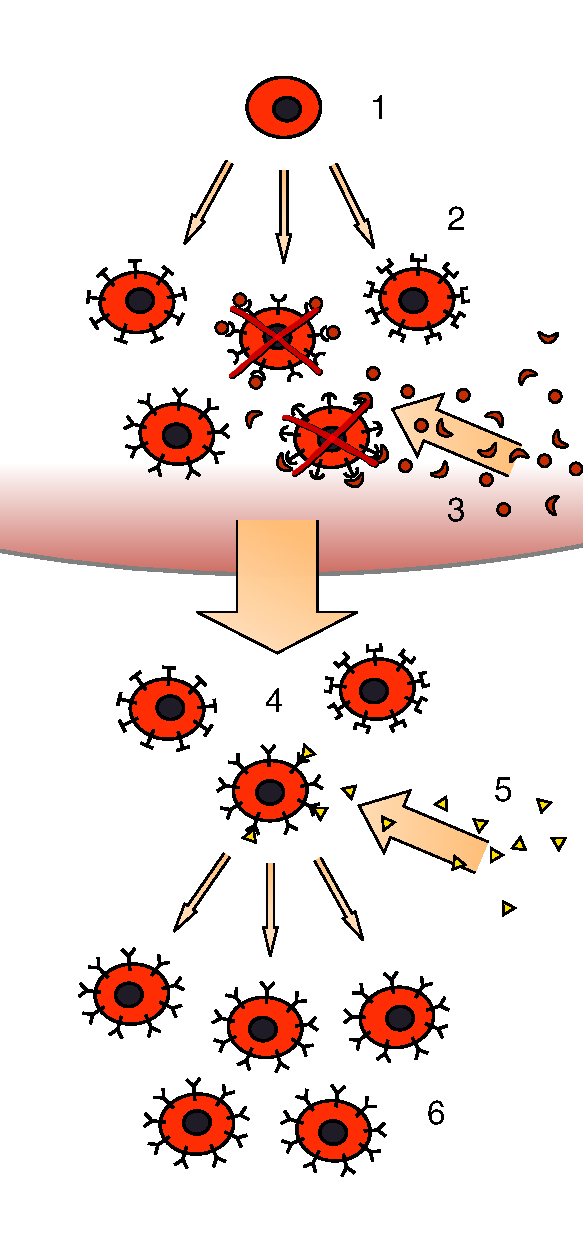
\includegraphics[width=0.3\textwidth]{img/clonalSelection.pdf}
\end{center}
\caption{Ejemplo de una selección clonal de linfocitos}
\label{fig:clonalSelection}
\end{figure}

Se señala la descripción de la figura~\ref{fig:clonalSelection} se detalla a continuación:
\emph{(1)} Una célula madre hematopoyética se somete a la diferenciación y
la reordenación genética para producir \emph{(2)} linfocitos inmaduros con
varios receptores de antígenos distintos.
Aquellos que se unen a \emph{(3)} antígenos de los tejidos del propio cuerpo
son destruidas, mientras que el resto madura y se convierten en \emph{(4)} linfocitos
inactivos. La mayoría de ellos nunca encontrarán un patógeno correspondiente \emph{(5)}
antígeno exterior, pero aquellas que se activan y producen (6) muchos clones de sí mismos.

\subsection{Algoritmo de la Selección Clonal}



Siguiendo el principio de selección clonal y el proceso de maduración de la afinidad, postulado por De Castro~\cite{decastro} se puede describir el algoritmo de selección clonal de la siguiente forma:
\begin{figure}[h!]
\begin{center}
%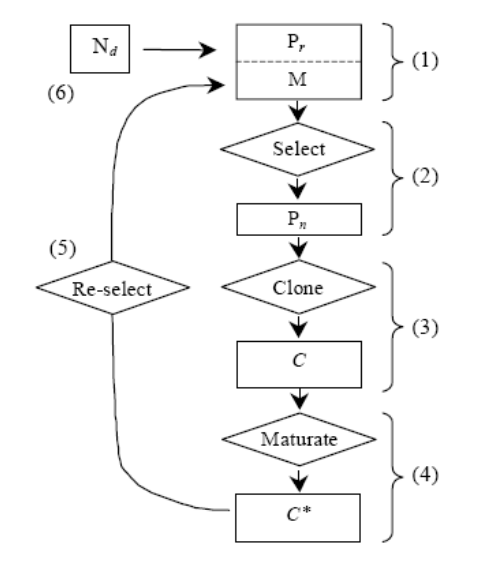
\includegraphics[width=0.5\textwidth]{img/algoritmo}
\end{center}
\caption{Diagrama del algoritmo de la selección clonal}
\label{fig:algoritmo}
\end{figure}

Siendo la explicación de los pasos de la figura~\ref{fig:algoritmo} la siguiente:
\begin{enumerate}
    \item Generar un conjunto (P) de soluciones candidatas, compuesto de células de memoria (M) añadidas a la población restante (Pr), teniendo entonces $P = Pr + M$
    \item Determinar los $n$ mejores individuos (Pn) de la población (P), basado en una medida de afinidad.
    \item Clonar (reproducir) estos $n$ mejores individuos de la población, dando origen a una población temporal de clones (C).
    \item Someter la población de clones a un esquema de hiper-mutación (proporcional a la afinidad del anticuerpo). Una población de anticuerpos maduros es generada (C*).
    \item Seleccionar nuevamente los mejores individuos de (C*) para componer el conjunto de memoria. (Algunos reemplazos desde (C*) a (P), debido a la mejora)
    \item Reemplazar los $d$ anticuerpos con menor afinidad de la población, manteniendo la diversidad.
\end{enumerate}


\label{sec:tecnica}

\subsection{Algoritmo propuesto}
\subsubsection{Componentes}
% Descripción los componentes que se probaron.
% Ej. AIS: Operadores de seleccion,
%		   Operadores de clonacion,
%		   Operadores de reemplazo,
%		   Movimientos,
%		   Funciones objetivos, etc.
% Resultados de las pruebas realizadas (tablas o gráficos). Ejemplo:
%	\begin{table}
%	\centering
%	\begin{tabular}{| l | c | c | c | c |}
%	\hline
%	 fobj & primeros & ruleta & torneo & random \\
%	\hline
%	 instancia 1 & 33000 &  31000 & 30000 & 40000 \\
%	\hline
%	 instancia 2 & 56000 &  45000 & 47000 & 60000 \\
%	\hline
%	\end{tabular}
%	\caption{Resultados pruebas Operadores de selecci\'on}
%	\end{table}

Debido a la cantidad de elementos que varían para probar el desempeño
del algoritmo, se ha establecido un conjunto de parámetros que hacen
referencia a la ejecución "base" del algoritmo.
\begin{itemize}
	\item Repertorio Inicial: Arreglado (Cumpliendo restricciones duras).
	\item Selección de Clones: Mejores (Considerando la población actual y la de clones).
	\item Movimiento: Swap al 40\%.
	\item Reemplazo: Peores.
	\item Clonación: Mediante fórmula (explicada más adelante).
\end{itemize}

\begin{enumerate}
	\item \textbf{Repertorio Inicial}

		El repertorio inicial, se ha generado de dos formas para poder establecer una mejor opción.
		\begin{itemize}
			\item \emph{Aleatorio:}
	
				Para éste caso, la población se ha generado completamente aleatoria, es decir,
				se ha creado una secuencia de vehículos considerando los tipos que el problema
				requiere, pero no se ha verificado que cada tipo de vehículo sea la cantidad
				necesitada por el problema.
			\item \emph{Arreglado:} 
				
				Se ha generado la población inicial con una lista de vehículos que contiene
				la cantidad exacta de los tipos necesitados por el problema, los cuales
				han sido desordenados, para dejar satisfechas en todo momento las restricciones
				blandas.
		\end{itemize}

	\item \textbf{Operador de Selección}
		% 1. Seleccion por ruleta
		La cantidad de elementos seleccionados corresponde al $selRate$ que consiste en una cantidad que corresponde
		al $40\%$ de la población.

		\begin{itemize}
			\item \emph{Roulette wheel:}
 
				Al momento de seleccionar individuos para realizar la clonación, se utilizó la conocida técnica llamada
				\emph{roulette wheel}, para una Función Objetivo que minimiza.
				
				El procedimiento es bien simple, sólo tenemos que considerar el \emph{fitness} de cada linfocito y calcular un
				\emph{fitness relativo} de la siguiente forma:
				
				$$relativeFitness_{i}\ = \frac{f_{min} + f_{max} - f_{i}}{\sum\limits_{i=0}^{sizePop} (f_{min} + f_{max} - f_{i}}$$
				
				Donde $f_{max}$ equivale al \emph{fitness} del mejor linfocito,
				$f_{min}$ equivale al \emph{fitness} del peor linfocito y
				$f_{i}$ equivale al \emph{fitness} del i-ésimo linfocito de nuestra población.
				
				La suma de todos los \emph{fitness relativo} equivale a $1$.
					
				Luego de que cada linfocito posee su \emph{fitness relativo}, se procede a calcular un \emph{fitness acumulativo},
				es decir, ir sumando las probabilidades para generar un rango entre $0$ y $1$ con todas nuestras probabilidades.
					
				Una vez se tiene el \emph{fitness acumulativo} listo, se procede a obtener un número aleatorio entre $0$ y $1$,
				para que luego sea ubicado en nuestro rango, y así el linfocito que salga escogido con éste número aleatorio, será
				elegido para pasar ahora a la transformación.
		
				% 2. Seleccionar siempre los mejores
				% Pendiente
			\item \emph{Mejores:}
				La selección de clones se realiza considerando todos los individuos de la población inicial y también
				la lista de clones que ya han sido hipermutados, por lo cual detrás del procedimiento está inmerso una
				esencia de elitismo, pues no estamos perdiendo los buenos elementos que hayan quedado en la población
				antes de la clonación e hipermutación.

		% Tabla comparativa
		\end{itemize}
	\item \textbf{Operador de Clonación}
		\begin{itemize}
			% 1. Clonación una cantidad aleatoria de veces
			% Pendiente
			\item \emph{Fórmula:}

				Se ha tomado la esencia de la fórmula propuesta por De Castro~\cite{decastro},
				en el cual consideramos tres elementos: ``factor de clonación ($\beta$)~\footnote{$clonationRate$
				corresponde al tamaño del $40\%$ de la población}'', ``Total de anticuerpos($N$)'' y
				``Afinidad (ranking) ($a$)''.
				La relación está dada por un número $m$ que equivale a la cantidad de clones que se generarán
				para cada anticuerpo ordenados por afinidad, partiendo del mejor al peor.
				$$m\ =\ \lceil\frac{\beta \cdot N}{a}\rceil$$

				Con ésto estamos siguiendo la idea central del algoritmo, pues estamos favoreciendo a que se clonen más
				los mejores elementos de nuestra población.
				
			% 2. Clonacion por fórmula
			% Pendiente
			\item \emph{Secuencia fija:}
			
				En éste caso, se considera una cantidad $n$ que consiste al $50\%$ de la diferencia entre el total de la población
				y los elementos que han sido seleccionados para la clonación (elementos nulos), luego utilizan por cada loop
				dicha cantidad, pero descontando el $10\%$ del total de la población, por lo que vamos obteniendo una cantidad
				de clones que va en disminución, dando prioridad a los mejores clones.
			
		\end{itemize}
		% Tabla comparativa
	\item \textbf{Operador de Reemplazo}
		Para mantener la diversidad en nuestra población e intentar escapar de los óptimos locales,
		se utiliza un $replaceRate$ que corresponde a la cantidad del $60\%$ del tamaño de la población.

		Los nuevos elementos son generados cumpliendo las restricciones duras, para obtener nuevos
		elementos un poco mejores en comparación a la creación aleatoria.
		\begin{itemize}
			% 1. Reemplazo aleatorio
			% Pendiente
			\item \emph{Aleatorio:}
 
				Se realiza el reemplazo en posiciones aleatorias de la población de los nuevos elementos
				generados.

			% 2. Reemplazo de los más malos
			% Pendiente
			\item \emph{Peores:}
				Se realiza el reemplazo en los peores elementos de la nueva población a utilizar.

		\end{itemize}
		% Tabla comparativa
	\item \textbf{Movimiento}
		En éste caso se realiza un \emph{swap}, pero como cada individuo es del orden de $200$, $300$ y $400$ autos,
		se realiza una cantidad de \emph{swap} equivalente al $40\%$ de la cantidad de autos.
	
		Para ver que elementos hacen el \emph{swap}, se eligen aleatoriamente dos elementos para intercambiar.~\footnote{
		Éste proceso se podría mejorar, estudiando a fondo que swaps nos convienen más, para obtener siempre mejores
		resultados}
\end{enumerate}


Respecto a los gráficos comparativos de cada situación,
se ha realizado 5 configuraciones distintas, para ver la diferencia en el rendimiento:
\begin{enumerate}
	\item Normal:

		\begin{itemize}
			\item Generación de población: Cumpliendo restricciones duras.
			\item Selección de clones: Selección de los mejores.
			\item Reemplazo al término de iteración:  Se reemplazan los peores.
			\item Tipo de clonación: Mediante fórmula.
		\end{itemize}
	\item Población aleatoria:

		\begin{itemize}
			\item Generación de población: \textbf{Rompiendo restricciones duras}.
			\item Selección de clones: Selección de los mejores.
			\item Reemplazo al término de iteración:  Se reemplazan los peores.
			\item Tipo de clonación: Mediante fórmula.
		\end{itemize}

	\item Selección ruleta:

		\begin{itemize}
			\item Generación de población: Cumpliendo restricciones duras.
			\item Selección de clones: \textbf{Selección mediante ruleta}.
			\item Reemplazo al término de iteración:  Se reemplazan los peores.
			\item Tipo de clonación: Mediante fórmula.
		\end{itemize}

	\item Reemplazo aleatorio:

		\begin{itemize}
			\item Generación de población: Cumpliendo restricciones duras.
			\item Selección de clones: Selección de los mejores.
			\item Reemplazo al término de iteración:  \textbf{Se reemplazan aleatoriamente}.
			\item Tipo de clonación: Mediante fórmula.
		\end{itemize}

	\item Secuencia Fija:

		\begin{itemize}
			\item Generación de población: Cumpliendo restricciones duras.
			\item Selección de clones: Selección de los mejores.
			\item Reemplazo al término de iteración:  Se reemplazan los peores.
			\item Tipo de clonación: \textbf{Secuencia fija}.
		\end{itemize}

\end{enumerate}

Los resultados obtenidos y graficados corresponden al \emph{promedio}, \emph{desviación estándar},
\emph{valores mínimos}, \emph{valores máximos} y \emph{tiempo de ejecución}.


Ver anexo~\ref{sec:anexo}.

\label{sec:componentes}

\subsubsection{Algoritmo Final}
% Pseudo codigo del algoritmo final
%  (con los componentes elegidos a traves de las pruebas y su criterio).
% En lo posible adjuntar una tabla de los resultados encontrados por
%  su algoritmo y otros algoritmos de la literatura
%  (no es importante que sean buenos, es solo para comparar en que punto se encuentra). 

Las opciones utilizadas en el algoritmo, son las que conforman la configuración \emph{Normal}
previamente señalada.

\begin{verbatim}
    Inicio
    g <- 0 // numero de generaciones
    Leer datos de entrada
    Población <- Generar población inicial
    Evaluar población

    Mientras g < GENS
        Limpiar poblaciones
        Seleccionar individuos a clonal (ruleta)
        Clonación (fórmula)
        Hipermutación mediante Swap
        Evaluar población mutada
        Selección de clones (Mejores)
        Inserción de clones en nueva población
        Generar elementos nuevos aleatorios
        Inserción de elementos nuevos al población
        g <- g + 1
    Fin Mientras

    Imprimir resultados
    Fin
\end{verbatim}


\label{sec:algoritmo}

\section{Bibliografía}
%\bibliography{informe2}
\end{document} 
